\documentclass[border=5pt]{standalone}
\usepackage{tikz}
\usepackage{amsmath}
\usetikzlibrary{calc, positioning, arrows.meta, 3d}
\begin{document}
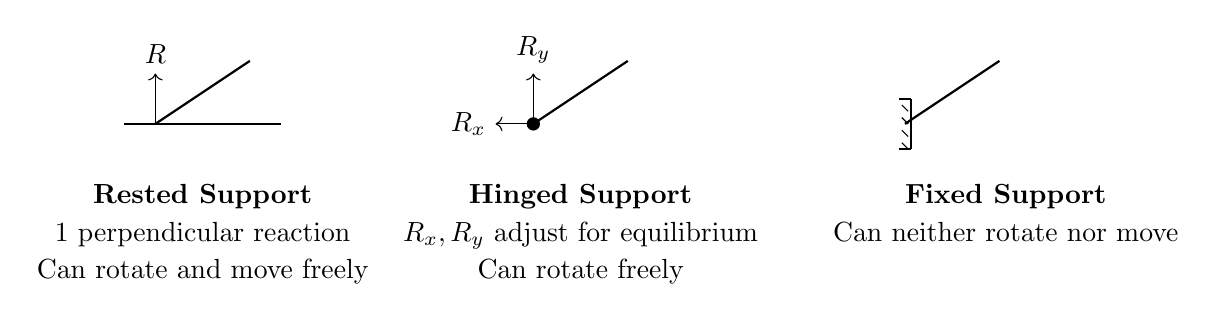
\begin{tikzpicture}[scale=0.8]
% Case 1: Rested Support
\begin{scope}[xshift=0cm]
% Draw rod at angle
\draw[thick] (0,0) -- (1.5,1);
% Draw support
\draw[thick] (-0.5,0) -- (2,0);
% Forces
\draw[->] (0,0) -- (0,0.8) node[above] {$R$};
\node[below] at (0.75,-0.8) {\textbf{Rested Support}};
\node[below] at (0.75,-1.4) {1 perpendicular reaction};
\node[below] at (0.75,-2) {Can rotate and move freely};
\end{scope}

% Case 2: Hinged Support
\begin{scope}[xshift=6cm]
% Draw rod at angle
\draw[thick] (0,0) -- (1.5,1);
% Draw hinge with rotation symbol
\fill (0,0) circle (3pt);
% Forces
\draw[->] (0,0) -- (0,0.8) node[above] {$R_y$};
\draw[->] (0,0) -- (-0.6,0) node[left] {$R_x$};

% Add moment equation
\node[below] at (0.75,-0.8) {\textbf{Hinged Support}};
\node[below] at (0.75,-1.4) {$R_x, R_y$ adjust for equilibrium};
\node[below] at (0.75,-2) {Can rotate freely};
\end{scope}

% Case 3: Fixed Support
\begin{scope}[xshift=12cm]
% Draw rod at angle
\draw[thick] (-0.1,0) -- (1.4,1);
% Draw fixed support
\draw[thick] (-0.2,-0.4) -- (0,-0.4);
\draw[thick] (-0.2,0.4) -- (0,0.4);
\draw[thick] (0,-0.4) -- (0,0.4);
\foreach \y in {-0.3,-0.1,0.1,0.3} {
  \draw (-0.15,\y) -- (-0.05,\y-0.1);
}
% Forces and moment
\node[below] at (1.5,-0.8) {\textbf{Fixed Support}};
\node[below] at (1.5,-1.4) {Can neither rotate nor move};
\end{scope}
\end{tikzpicture}
\end{document}
